%---------------------------------------------------------------------------------------------------
% Bahnplanung
%---------------------------------------------------------------------------------------------------
\DeclareInputText
\newpage
\chapter{Bahnplanung}
Die Navigation, also das effiziente und kollisionsfreie Bewegen im Raum, gehört zu den Hauptaufgaben von autonomen mobilen Robotern. Um, zum Beispiel Produktionsstraßen zukunftsfähig und effizienter zu gestalten, müssen die Robotinos konkreten Aufgaben wie \glqq Fahre zum Zielpunkt XY und nehme das Werkstück auf\grqq{} übernehmen und abarbeiten können. Dazu muss der Robotino zu jeder Zeit folgende Fragen beantworten können: \glqq Wo befinde ich mich? Wo muss ich hin? Wie gelange ich dort hin?\grqq (Mohamed Oubbati Einführung in die Robotik)
Anhand dieser Fragen lässt sich die Bahnplanung in drei Bereiche unterteilen:
\begin{itemize}
\item \textbf{Lokalisierung:} Genau Positionsbestimmung des Robotinos im bekannten Raum
\item \textbf{Kartenerstellung:} Vom Roboter über Sensordaten erstellte oder durch Softwareimplementierung bekannte Karte des Raumes
\item \textbf{Trajektoriengenerierung:} Berechnung von Trajektorien vom Startpunkt zum Ziel
\end{itemize}
\section{Lokalisierung}
Eine Bahnplanung kann nur dann erfolgen, wenn der Roboter seine eigene Position zu jeder Zeit lokalisieren kann. 
In dem Fall des hier ausgearbeiteten Projektes erfolgt die Lokalisierung über Deckenkameras, die mittels UDP-Kommunikation den Robotinos ihre eigene Position, aber auch die der anderen Robotinos im bekannten Raum senden. Intern wurde über den Raum ein Koordinatensystem gelegt,so dass die genaue Position der Roboter in x- und y-Richtung ausgegeben werden kann. Zu diesem Zweck sind die Robotinos mit ArUco-Markern ausgestattet. Um ein zuverlässiges Gesamtsystem zu erschaffen und die Ausfallwahrscheinlichkeit zu minimieren, erfolgt die Lokalisierung zusätzlich über Positionsdaten des Gewerks 3 \glqq Regelung\grqq. Somit wird sichergestellt, dass bei ungenauen und nicht vorhandenen Kameradaten die Robotinoposition zu jeder Zeit bekannt ist und ein unterbrechungsfreier Ablauf des Prozesses gegeben ist. 
\section{Kartenerstellung}
Mit bekannten Karten und vom Roboter durch die Sensorik erstellte Karten helfen beim Wegfinden. Durch eine vorab implementierte Karte können Hindernisse und Sackgassen implementiert werden, die von dem Transportroboter gemieden werden müssen. Kennt der Robotino seine Umgebung durch eine Karte kann über Selbstlokalisierung ein optimaler Pfad generiert werden. Im Fall der vorliegenden Projektes muss der Roboter nicht durch willkürliches Fahren im Raum vorab eine Karte von unbefahrbaren Punkten sammeln. Den Robotinos sind die festen Hindernisse, das heißt Lager, Lade- und Werkstationen, auf Grund der implementierten Programmierung von vornherein bekannt.
\section{Trajektoriengenergierung}
Durch die Bahnplanung können kollisionsfreie Trajektorien von einem Start- zu einem Zielpunkt generiert werden. Als Trajektorie wird in der Physik der Bewergungsverlauf des Roboters als Kurve im Raum bezeichnet, also die Zustandsänderung relativ zum Koordinatensystem über die Zeit. Es werden Solltrajektorien berechnet, die dem Gewerk 3 \glqq Regelung\grqq über eine definierte Schnittstelle übergeben werden. Über diese Trajektorie wird der Robotino zum Ziel geführt.

Die Literatur bietet viele verschiedene Ansätze zur Berechnung des bestmöglichen Pfades und hängt von der projektspezifischen Aufgabenstellung und Definition von \glqq bester Pfad\grqq ab. \glqq Bester Weg\grqq wird im Allgemeinen mit kürzester Distanz assoziiert. Es kann aber auch andere Faktoren beinhalten, die angeben wie \glqq teuer\grqq ein Weg ist. Ist der Untergrund zum Beispiel schlecht befahrbar, so könnte es schneller sein einen Umweg zu fahren. Auch könnten kinematische und dynamische Eigenschaften des Roboters in die Definition mit eingehen, so dass Pfade vermieden werden, die Kurven beinhalten, die der Roboter nicht fahren kann. Auch Kriterien wie Energieeffizienz, Schnelligkeit und größtmöglicher Abstand zu Hindernissen haben je nach Aufgabenstellung eine andere Gewichtung bezüglich des Bahnplanungsansatzes.

%Beispielsweise wird bei der Aufgabenstellung \glqq Finde den schnellsten Weg zum Ziel\grqq ein anderer Berechnungsansatz der Bahnplanung verfolgt als bei \glqq Finde den energieeffizientesten Weg zum Ziel\grqq. Weitere Kriterien zum Auswählen eines Bahnplanungsansatzes könnten beispielsweise sein, immer den größtmöglichen Abstand zu Hindernissen zu fahren, die kürzeste Strecke zu finden oder Strecken nach Vorhersagbarkeit des Weges zu bewerten. Allgemein wird in der Bahnplanung zwischen globaler und lokaler Bahnplanung unterschieden. 

Im Nachfolgenden werden unterschiedliche Bahnplanungsansätze betrachtet und bewertet.
\subsection{Globale Bahnplanung}
Bei der globalen Bahnplanung, in der englischsprachigen Literatur auch bekannt als \glqq Map-Based Planing\grqq müssen dem Robotino der Raum und die sich darin befindlichen statischen Hindernisse und Sackgassen vollständig bekannt sein, um diese in jedem Fall zu vermeiden. Im Folgenden werden drei Möglichkeiten der globalen Bahnplanung beschrieben: 
\begin{itemize}
\item \textbf{Sichtbarkeits-Methode mit A*-Algorithmus}
\item \textbf{Occupancy Grid mit D*}
\item \textbf{Voronoi Roadmap Methode}
\end{itemize}

\subsubsection{Sichtbarbeitsgraph Methode mit A*}
Der Sichtbarkeitsgraph (engl. Visible graphs) ist eine Methode um den kürzesten Pfad zwischen zwei Punkten zu finden. 
Diese Methode setzt voraus, dass vorab Start- und Zielpunkt, so wie Eckpunkte der statischen Hindernisse klar definiert und bekannt sind.  
Die Eckpunkte der Hindernisse werden dann durch eine Kante verbunden, wenn eine gerade Verbindungslinie gezogen werden kann ohne andere Hindernisse zu schneiden. Dadurch werden Eckpunkte zu Knotenpunkten. Die Hindernisse mit den Verbindungslinien ist in Abbildung 3.1 Sicherheitsgraph dargestellt. Die dicke schwarze Linie ist der resultierende optimale Pfad. 
\begin{figure}[h]
	\centering	
	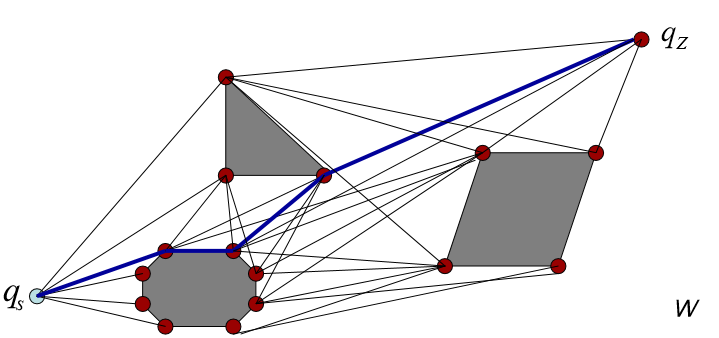
\includegraphics{Sichtbarkeitsgraph.png}
	\caption{Beispiel Sichtbarkeitsgraph, schwarze Blöcke entsprechen Hindernissen, linien entsprechen Kantenverbindung zwischen Knotenpunkten, dicke linie entspricht optimalem Pfad}
	\label{fig:Sichtbarkeitssgraph}
\end{figure}

Durch Einsatz der A*-Methode kann so der optimale Pfad bestimmt werden. Die Kanten zwischen zwei Knotenpunkten werden von dem Algorithmus je nach Anforderung, beispielsweise kürzester Weg, gewichtet. Je größer diese Gewichtung ist, desto weiter Weg befindet sich der Knotenpunkt am anderen Ende der Kante. Die direkte Entfernung eines Knotenpunktes zum Zielpunkt wird geschätzt, so dass die Knoten ebenfalls eine Gewichtung bekommen. 

Vom Zielpunkt aus werden nun alle Knoten betrachtet, die über eine Kante erreicht werden können. Der aus der Betrachtung hervorgehende Knotenpunkt, der die geringste direkte Entfernung zu Ziel aufweist, wird als nächstes untersucht. Die anderen werden gespeichert und im weiteren Verlauf mit Konten hinsichtlich ihrer Gewichtung verglichen. Punkte, die bereits betrachtet wurden, werden  als \glqq untersucht \grqq markiert. Dieses Verfahren wiederholt sich so lange bis der optimale Pfad gefunden wurde. 

Ein Vorteil dieser Methode ist, dass immer der optimale Pfad vom Start zum Ziel gefunden wird. Nachteile sind jedoch, dass der Pfad immer direkt an den Ecken und Kanten der Hindernisse entlang führt. Außerdem kann ein sehr großer Graph entstehen, der berechnet werden muss. 

\subsubsection{Occupancy Grid mit D*}
Wie der Name \glqq Occupancy Grid\grqq vermuten lässt, wird der Raum in ein Gitternetz unterteilt. Jede entstehende Zelle kann mit einer \glqq 1\grqq für \glqq belegt\grqq und \glqq 0\grqq für \glqq frei\grqq versehen werden. Dadurch entsteht ein Raum im dem Hindernisse und freier Raum zum Fahren klar definiert sind. 

Der D*-Algorithmus verändert die Bewertung der einzelnen Zellen mit einem neuen Wett, der die \glqq Kosten\grqq der Zelle repräsentiert. Zellen, die zu einem Hindernis gehören werden mit \glqq $ \infty $\grqq gewichtet. Mit diesem Algorithmus wird immer der optimale Pfad gefunden. Je nach Aufgabenstellung kann diese Gewichtung zum Beispiel Distanz oder Zeit bedeuten. 

Ein Vorteil dieser Methode ist, dass der Weg schrittweise neu geplant werden kann. Sollte sich der Raum anders sein, als zuvor in dem Gitternetz eingetragen, eine Zelle beispielsweise teurer als geplant, so kann stufenweise ein besserer Pfad gefunden werden. Die Berechnung des neuen Weges erfordert nicht so viel Rechenleistung eine komplett neue Wegplanung, da nur die Zellen in direkter Umgebung betrachtet werden. Die Anfangsberechnung ist hingegen sehr rechenintensiv. 

\subsubsection{Voronoi Roadmap Methode}

\subsection{Lokale Bahnplanung}
Die lokale Bahnplanung betrachtet nur das direkte Umfeld des Roboters. Ziel ist hierbei die reaktive Kollisionsvermeidung.